\chapter{Estimation ponctuelle de la densité de probabilité}
\section{Introduction}
La modélisation stochastique de systèmes technologiques complexes et de phénomènes scientifiques nécessite souvent une estimation précise des densités de probabilité. L'utilisation d'un estimateur fiable améliore les performances de ces systèmes ou permet une meilleure compréhension des phénomènes étudiés. Il existe différentes méthodes pour estimer ces densités, des méthodes paramétriques et d’autres non-paramétriques. Dans ce chapitre nous allons nous focaliser sur les méthodes non-paramétriques, notamment la méthode de l’histogramme, la méthode du noyau, la méthode des fonctions orthogonales \shortcite{hall1982} et la méthode du noyau difféomorphisme \shortcite{troudi2021generalised} qui permet de limiter l'effet du phénomène de Gibbs. 

\setlength{\parindent}{0 cm}
Cependant, comme pour la méthode du noyau conventionnel, il est important d’optimiser la valeur du paramètre de lissage noté  $h_n$ , pour garantir une bonne qualité de l’estimation. Une étude de convergence a été menée pour optimiser ce paramètre au sens de l’Écart Quadratique Moyen 
(EQM). Plusieurs méthodes ont été proposées pour la sélection du pas optimal les principales étant la méthode "rule of thumb" (règle empirique) \shortcite{silverman1986}, la méthode de la validation croisée et ses variantes \shortcite{bowman1984}\shortcite{hall1992} la méthode plug-in \shortcite{hall1987}, la méthode des contrastes\shortcite{mugadi2004}

\setlength{\parindent} {0 cm}
La première section explique la densité de probabilité. Puis, nous allons voir les méthodes paramétriques et non-paramétriques d’estimation de la densité.  Nous nous intéressons aux méthodes d’optimisation du paramètre de lissage et plus particulièrement à l’algorithme itératif du Plug-in. La quatrième section est dédiée à la présentation de la méthode que nous allons utiliser plus tard. 
\section{Formalisation de l'estimation de la densité de probabilité }
Soit  $X$  une variable aléatoire et  $F_X$ sa fonction de répartition, s’il existe une fonction $f_x$ positive de $L^{1}$$(\Omega)$ telle que : 


\begin{equation}
   \forall x \in \Omega, F_x(x) = \int_{-\infty}^{x} f_x(u)\,du
\end{equation}
\myequations{Equation \ref{eq:Eq1}}

alors  $f_x$    s’appelle la densité de probabilité de la variable aléatoire $X$.  $f_x$ vérifie :
\begin{equation}
\int_{-\infty}^{+\infty} f_x(x)\,dx = 1
\end{equation}
\myequations{Equation \ref{eq:Eq2}}
Lorsque nous connaissons la densité de probabilité  $f_x$  de $X$, il est possible de calculer la probabilité d’appartenance d’une variable aléatoire $X$ à n’importe quel ensemble 
\begin{equation}
A\subseteq \Omega : P(X<A)=\int_{-\infty}^A f_x(x)\,dx
\end{equation}
\myequations{Equation \ref{eq:Eq3}}
\subsection{Normes d'évaluation de la densité de probabilité}
Un estimateur de la densité de probabilité f est une application $f_N$ telle que :
\begin{equation}
{\hat f}{N}: \psi^n \rightarrow \mathbb{R}^\psi \\ (X_1,\dots,X_n) \mapsto {\hat f}{N}(X_1,\dots,X_n;x) = {\hat f}_{N}(x)
\end{equation}
\myequations{Equation \ref{eq:Eq4}}
La qualité d'un estimateur est évaluée en mesurant l'écart entre les densités réelles et estimées.
\begin{itemize}
  \item Norme de convergence simple:
\begin{equation}
\|{\hat f}_{N} - f\|_x = |{\hat f}_{N}(x) - f(x)|\\\shortcite{apostol1974norme}
\end{equation}
\myequations{Equation \ref{eq:Eq5}}
  \item Norme de convergence uniforme : 
  \begin{equation}
\|{\hat f}_{N} - f\|_{\infty} = \sup|{\hat f}_{N}(x) - f(x)|\\\shortcite{apostol1974norme}
\end{equation}
\myequations{Equation \ref{eq:Eq6}}
  \item Norme de convergence $L^2$  :
  \begin{equation}
\|{\hat f}_{N} - f\|_{L^2} = \int |{\hat f}_{N}(x) - f(x)| \, dx
\\\shortcite{john1991partial}
\end{equation}
\myequations{Equation \ref{eq:Eq7}}
\end{itemize}


\section{Méthodes paramétriques }

Les méthodes paramétriques d'estimation de densité de probabilité sont souvent basées sur la connaissance de la forme fonctionnelle de la distribution sous-jacente et sur l'estimation de ses paramètres.
\subsection{La méthode des moments}
Soit $f: I \rightarrow \mathbb{R}$ continue sur un intervalle $I$ (non réduit à un point) de $\mathbb{R}$. Étant donné un entier naturel $r$, le moment d'ordre $r$ de $f$ est défini par :

\begin{equation}
m_r(f) \triangleq {\int_{x\in I}} x^r f(x)\,dx
\end{equation}
\myequations{Equation \ref{eq:Eq8}}
La méthode des moments \shortcite{pearson1894contributions,aslam2005moment} est une méthode paramétrique couramment utilisée pour estimer les paramètres d'une distribution de probabilité. Elle consiste à égaler les moments théoriques de la distribution (calculés à partir des paramètres inconnus) aux moments empiriques calculés à partir des données observées.\\
Plus précisément, pour une distribution de probabilité ayant des paramètres inconnus $\theta_1$, $\theta_2,...,\theta_k$  les moments empiriques d'ordre $k$ sont définis comme :
\begin{equation}
m_k = \frac{1}{n} \sum_{i=1}^n (x_i - m)^k
\end{equation}
\myequations{Equation \ref{eq:Eq9}}
 
Avec

$m = \frac{1}{n} \sum_{i=1}^n x_i$
\,,n est le nombre d'observations.

Par exemple, pour la distribution normale, les deux premiers moments théoriques sont :
\newline
$\mu_1 = \theta_1$
\newline
$\mu_2 = \theta_2$
\newline
\newline
La méthode des moments consiste alors à résoudre les équations suivantes pour les paramètres inconnus :
\newline
$m_1 = \mu_1$
\newline
$m_2 = \mu_2$
\subsection{La méthode du maximum de vraisemblance}
\begin{Definition}
La fonction $L_n: (x_1, x_2, \dots, x_n; \theta) = \prod_{i=1}^n P_{\theta}(X_i = x_i)$, pour des $X_i \rightarrow L(\theta)$, s'appelle la \textbf{vraisemblance} de la loi $L$. La variable aléatoire obtenue en appliquant la fonction $(x_1, x_2, \dots, x_n) \mapsto \operatorname{Argmax}_{\theta}{L(x_1, x_2, \dots, x_n; \theta)}$ appliquée au $n$-échantillon $(X_1, \dots, X_n)$ s'appelle l'\textbf{estimateur au maximum de vraisemblance} du paramètre $\theta$ de la loi $L(\theta)$ \cite{casella2002statistical}.
\end{Definition}
La méthode du maximum de vraisemblance consiste à trouver les valeurs des paramètres du modèle qui maximisent la vraisemblance des données observées. En d'autres termes, il s'agit de trouver les valeurs des paramètres qui rendent l'échantillon observé le plus probable sous le modèle donné. Une fois que les valeurs des paramètres ont été trouvées, la qualité de l'ajustement du modèle aux données peut être évaluée en calculant la fonction de vraisemblance maximale et en comparant les prévisions du modèle avec les données observées.
\subsection{La méthode de Pearson}
La méthode de Pearson \cite{pearson1894contributions,su2021generalized} peut être utilisée pour estimer la densité de probabilité d'une distribution univariée ou multivariée. Pour une distribution univariée, la fonction de densité de probabilité choisie est généralement une distribution normale ou une distribution de Student. Pour une distribution multivariée, la fonction de densité de probabilité choisie est généralement une distribution normale multivariée ou une distribution de Student multivariée.

La méthode de Pearson consiste en trois étapes :
\begin{enumerate}
\item Calculer les moments de la distribution à partir des données.
\item Choisir une fonction de densité de probabilité qui dépend de certains paramètres. Les paramètres sont choisis pour que la fonction de densité de probabilité corresponde aux moments de la distribution calculés à l'étape 1.
\item Estimer les paramètres de la fonction de densité de probabilité en utilisant les moments calculés à l'étape 1.
\end{enumerate}

NB : La méthode de Pearson nécessite la sélection d'une distribution de probabilité paramétrique, alors que la méthode des moments ne nécessite pas cette étape.

\section{Méthodes non-paramétriques}
Le principal avantage de l'estimation non-paramétrique de la densité de probabilité c'est qu’il n’est pas nécessaire d’avoir une connaissance préalable sur le type de la loi. Il existe plusieurs méthodes que nous développons ci-dessous.
\subsection{Méthode de l’histogramme}
L'histogramme de densité est une méthode simple d'estimation consistant à diviser l'espace des valeurs possibles de la variable aléatoire $X$ en intervalles égaux, appelés bins. Le pas de l'histogramme, noté $h_N$, est la mesure de ces intervalles.
\newline
On choisit un point d’origine $t_0$ et une longueur de classe $h_N$ ($h_N > 0$). Les bins sont définies par :
\begin{equation}
I_k=[t_k,t_{k+1} [\text{ avec } k \in \mathbb{Z}
\end{equation}
\myequations{Equation \ref{eq:Eq10}}
$\text{Sachant que : } t_{k+1}=t_k+h_N$
\newline
Si nous notons le nombre d’observations dans une classe $I_k$ par $\hat{N}(k)$, l’estimateur du type histogramme de densité (dans chaque bin) s’écrit :
\begin{equation}
{\hat f}_{N}(x) = \frac{\hat{N}(k)}{N h_N} = \frac{1}{N h_N} \sum_{i=1}^n [t_k, t_{k+1}\lbrack\,, X_i, \forall x \in I_k
\end{equation}
\myequations{Equation \ref{eq:Eq11}}
Le choix du pas (paramètre de lissage $h_N$) est critique. Un pas inférieur au pas optimal peut causer une estimation perturbée de la densité de probabilité (Figure 1.1). Un pas supérieur au pas optimal peut aussi causer une estimation trop lisse (Figure 1.1). Figure 1.2 représente l'estimation de densité de probabilité en utilisant $h_N$ optimal. 
\newline 
Même une variation de $10^{-3}$ peut causer ces problèmes.
\begin{figure}[!ht]
  \centering
  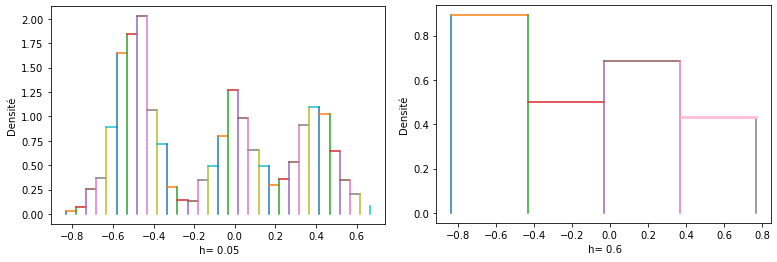
\includegraphics[width=\textwidth]{Figure 1.1.png}
  \caption{Différents histogrammes associés à un même ensemble de données avec différents paramètres de lissage}
  \label{fig:hneleveetbas}
\end{figure}
\begin{figure}[!ht]
  \centering
  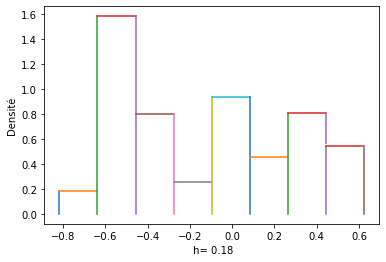
\includegraphics[width=13cm,height=8cm]{Figure 1.2.png}
  \caption{Estimation d’une densité de la probabilité par la méthode de
l’histogramme avec une valeur de pas optimal}
  \label{fig:figure2}
\end{figure}
\newpage

La figure (1.1) nous montre deux histogrammes basés sur le même ensemble de données et avec deux paramètres de lissage petit et grand. Un paramètre de lissage trop petit conduit à un histogramme plus découpé, tandis que l’autre donne un histogramme plus lisse comme le montre la figure (1.1).

\subsection{Méthode des fonctions orthogonales}
Pour cette méthode d’estimation non paramétrique, $f$ s’écrit sous la forme d’une série :
\begin{equation}
f(x) = \sum_{m=0}^{+\infty} a_m(f) e_m(x)
\end{equation}
\myequations{Equation \ref{eq:Eq12}}
Sachant que $e_m$ sont des fonctions orthogonales \newline et $a_m(f)$ les coefficients de Fourier de la densité à estimer $f$.
\newline
\newline
La méthode d’estimation consiste à tronquer la série qui s’écrit alors : 
\newline
$f_k (x)=\sum_{m=1}^k a_m (f)e_m (x)$
\newline
\newline
Puis à estimer les paramètres $(a_1 (f),...  ,a_k (f)$ , avec a$_m (f) = \int f(x) e_m (x)\,dx$, par :
\newline
${\hat a}_{m,N}=\frac{1}{N}\sum_{m=1}^{N}e_{m}(X_i)$
\section{Méthode de Noyau}
La méthode de noyau a été introduite pour la première fois par ROSENBLATT en 1956, puis développé par Parzen en 1962 pour décrire la fonction utilisée dans les méthodes non paramétriques. La méthode des noyaux consiste à associer une fonction $K(x)$ à chaque observation de l'échantillon, avec la seule restriction que son intégration sur tout le domaine de définition de $x$ doit être égale à 1. Certaines restrictions théoriques peuvent être imposées sur $K$, comme la symétrie ou la positivité sur tout le domaine de définition du noyau, mais elles sont principalement utilisées pour simplifier les développements théoriques.\newline L'estimation non paramétrique de la fonction de densité peut être vue comme la somme des fonctions $K$ de chaque observation sur tout le domaine.
\newline
Soit $K: \mathbb{R} \longrightarrow \mathbb{R}$, on dit que $K$ est un noyau si et seulement si :
\newline
$\int_{-\infty}^{\infty} K(u)du=1$
\newline
$K$ est dit positif si $K(u) \geq 0 \quad \forall u$
\newline
$K$ est dit symétrique si $K(u) = K(-u) \quad \forall u$
\newline
\newline
En pratique, les noyaux utilisés sont des noyaux d'ordre 2 ce qui implique que le noyau $K$ est lui-même une densité de probabilité. Des exemples de noyaux d'ordre 2 sont cités ci-dessous :
\begin{itemize}
    \item Le noyau rectangulaire : $K(u)=\frac{1}{2}1_{[-1,+1]}(u)$ (appelé aussi noyau de Rosenblatt)
    \item Le noyau triangulaire : $K(u)=(1-|u|)1_{[-1,+1]}(u)$
    \item Noyau d’Epanechnikov (parabolique) : $K(u)=\frac{3}{4}(1-u^2)1_{[-1,+1]}(u)$
    \item Le noyau Gaussien : $K(u)=\frac{1}{\sqrt{2\pi}}e^{-\frac{u^2}{2}}$
\end{itemize}
Les avantages des deux premières méthodes sont leur simplicité, car leur noyau est triangulaire et continu partout, ce qui permet une estimation continue. La troisième méthode est connue pour une propriété théorique d'optimalité, mais n'a pas d'importance pratique.
\newline
Voici quelques courbes de noyaux usuels présentées ci-dessous :

\begin{figure}[!ht]
  \centering
  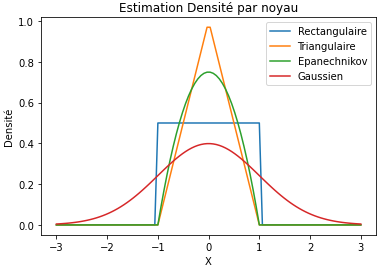
\includegraphics[width=\textwidth]{Figure 1.3.png}
  \caption{Les courbes des noyaux les plus communs}
  \label{fig:figure3}
\end{figure}

Un estimateur à noyau noté $f_n$ de la fonction $f$ est défini par : 
\begin{equation}
\hat{f}_N(x) = \frac{1}{N h_N} \sum_{i=1}^N K\left(\frac{x-X_i}{h_N}\right)
\end{equation}

\myequations{Equation \ref{eq:Eq13}}
Avec $(X_1, \dots, X_n)$ $N$ réalisations d’un échantillon et $K$ une densité de probabilité appelée noyau (Voir les exemples cités dans la partie précédente et \shortcite{parzen1962} pour une revue plus exhaustive). Ainsi, le noyau $K$ est centré sur le point $x$ dont on veut estimer l’image par $f$ : il s’agira de sommer les contributions des différents $x_i$ en normalisant par l’entité $h_N$ appelée "paramètre de lissage" ou plus simplement "pas".

\subsection{Description de l’estimateur à noyau }
Les différentes étapes de l'algorithme Plug-in sont détaillées ci-dessous :

\begin{enumerate}
\item \textbf{ Choix du noyau :}
Le choix du noyau dépend du problème à résoudre. Il existe plusieurs types de noyaux comme nous l'avons vu dans la partie précédente.

\item \textbf{ Fixation du paramètre de lissage :}
Cette étape est très importante, dans les parties suivantes nous allons voir les algorithmes qui vont nous aider à choisir le pas optimal.

\item \textbf{ Placement des noyaux sur les données :}
Pour chaque point de données, un noyau est placé autour de ce point. La forme et la taille du noyau dépendent du choix de noyau et du pas.

\item \textbf{ Normalisation de la densité de probabilité estimée :}
Pour que la densité de probabilité estimée puisse être interprétée comme une probabilité, elle doit être normalisée. Cela signifie que l'aire sous la courbe de densité de probabilité doit être égale à 1.

\item \textbf{Interprétation de la densité de probabilité estimée.}
\end{enumerate}
Les différentes étapes citées sont schématisées dans la figure 1.4 : 
\begin{figure}[!ht]
  \centering
  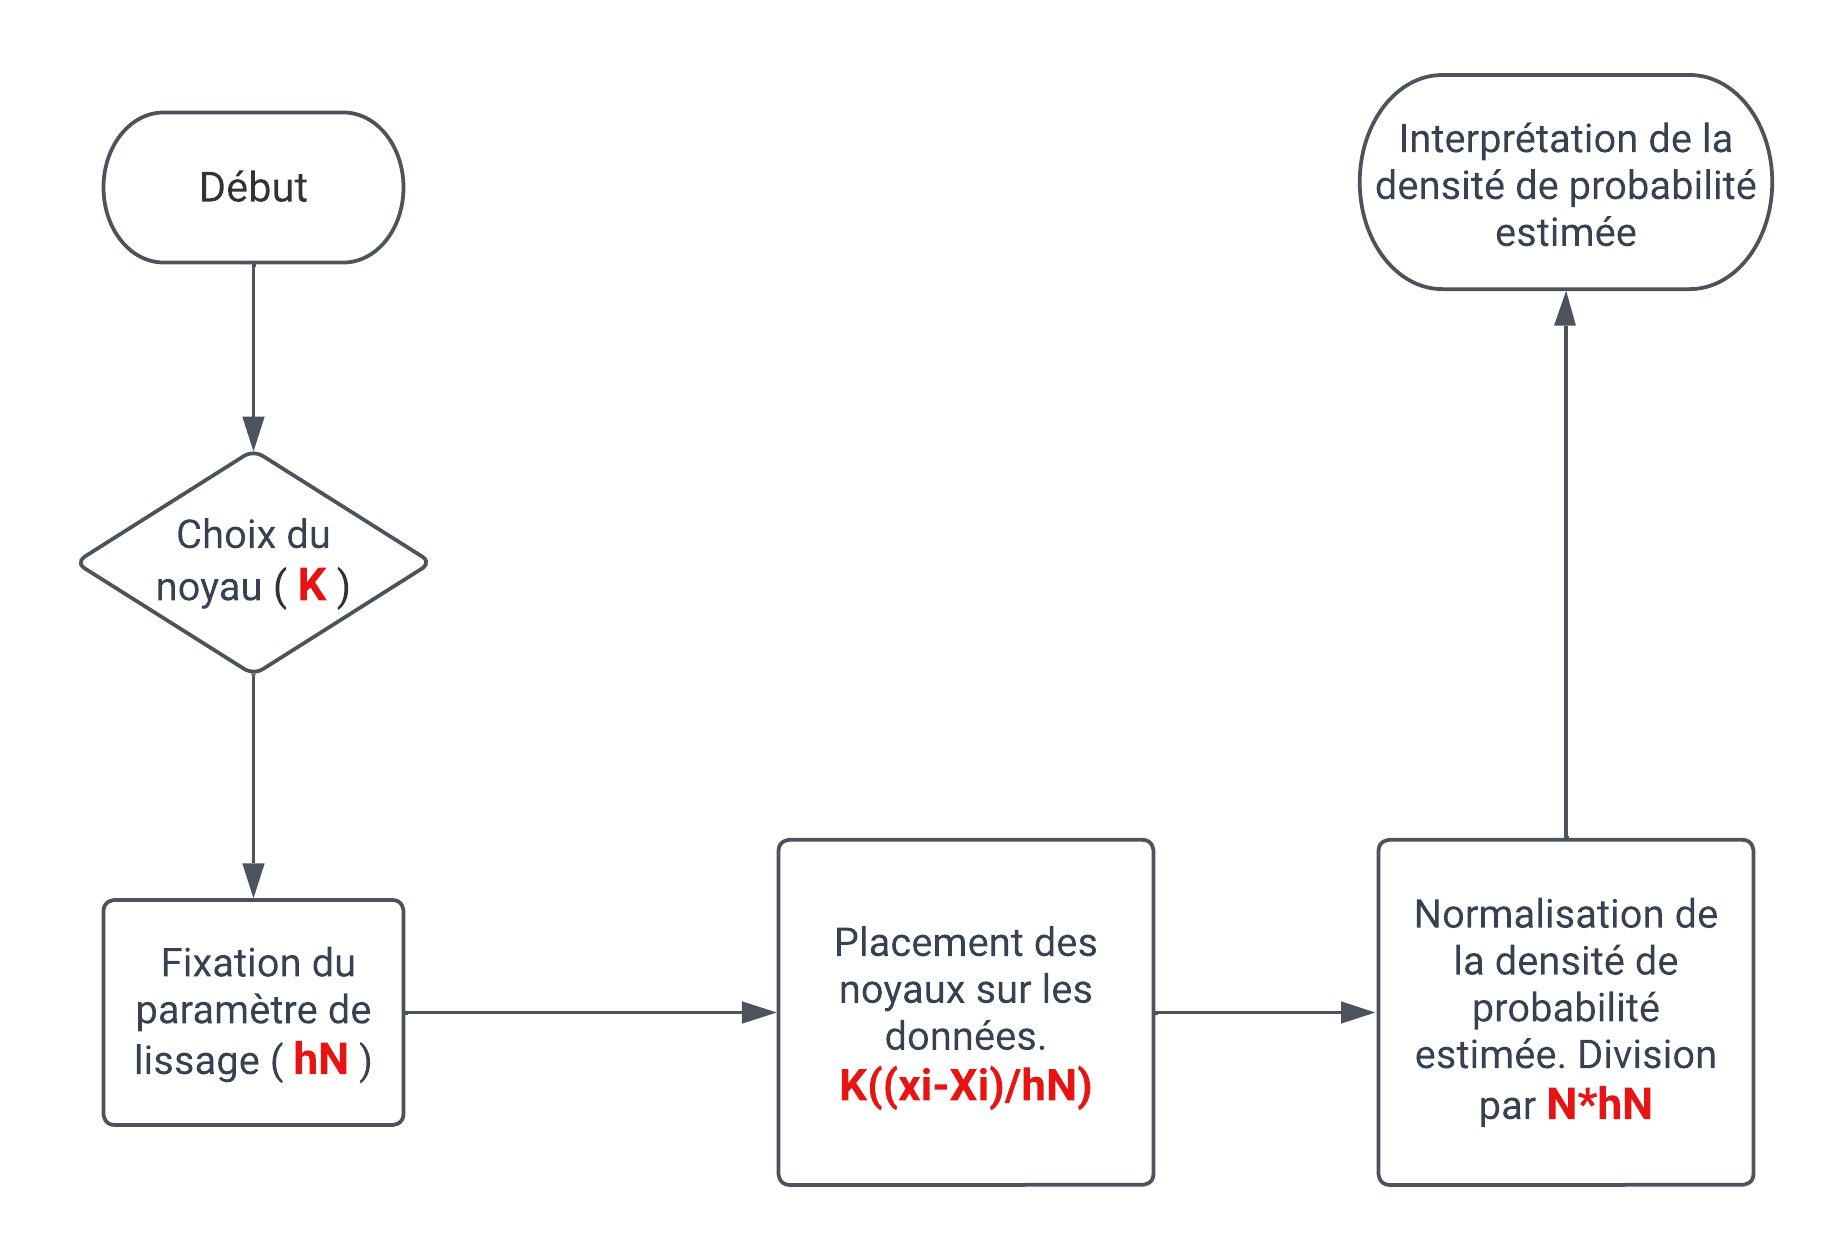
\includegraphics[width=14cm,height=10cm]{Figure 1.4.png}
  \caption{Schéma descriptif de l'estimateur à noyau}
  \label{fig:Schéma descriptif de l'estimateur à noyau}
\end{figure}
\newpage
Voici une implémentation en Python 3 de l'estimateur de noyau, permettant d’estimer la densité de probabilité d'un ensemble de données $X$ : \\
\begin{lstlisting}
X = generation_LN(m, s, n) 
P = 100
c = (2 * np.pi)**0.5
for NBI in range(1,10):
    hn = #valeur optimale
    valeur=2*2.23*(hn)**(-6)/500;
    Y = []
    Yk = []
    for k in range(P):
        yk = mini + (maxi-mini)*k/P
        Y.append(0)
        Yk.append(yk)
        for i in range(1,n):
            z = (yk-X[i]) / hn
            z = z**2
            z = -0.5*z
            z = np.exp(z)
            Y[-1] += z
        Y[-1] = Y[-1] / (c*n*hn)
    e = -100
        d = 100
    I = 0
    z = 0
    for k in range(1, P-2):
        z = (Y[k+1]-2*Y[k]+Y[k-1])
        I += z**2
    I = I + ((Y[P-2])**2 + (Y[P-2]-2*Y[P-3])**2) / (r**4)
return Y

\end{lstlisting}
Avec : \\
Les paramètres de la loi normale à générer sont $m$, $s$ et $n$ ( moyenne, écart-type, taille).
\newpage
\subsection{Paramètre de lissage}
Le choix des paramètres de lissage dans les méthodes du noyau pour estimer la densité de probabilité est un aspect important de ces méthodes. Le paramètre de lissage, également appelé paramètre de bande passante, contrôle la largeur du noyau utilisé pour lisser les données. Un paramètre de lissage plus élevé entraînera une estimation plus lisse de la densité de probabilité, mais pourrait masquer certains détails importants dans les données (Figure 1.5).\\ Un paramètre de lissage plus faible permettra une estimation plus détaillée de la densité de probabilité, mais pourrait entraîner une estimation plus bruitée (Figure 1.6). Il est donc important de trouver un compromis approprié entre le lissage et la résolution lors de la sélection des paramètres de lissage.
\begin{figure}[!ht]
  \centering
  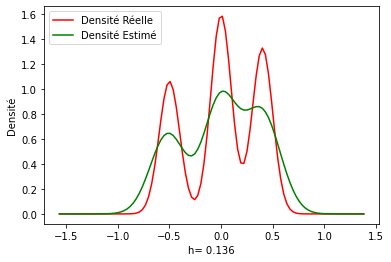
\includegraphics[width=13cm,height=10cm]{Figure 1.5.png}
  \caption{$h_N$  Élevé }
  \label{fig:$h_N$  Élevé}
\end{figure}
\begin{figure}[!ht]
  \centering
  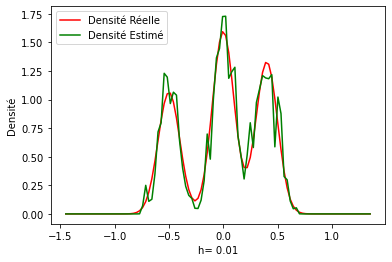
\includegraphics[width=13cm,height=8cm]{Figure 1.6.png}
  \caption{$h_N$  Faible }
  \label{fig:$h_N$  Faible}
\end{figure}
\begin{figure}[!ht]
  \centering
  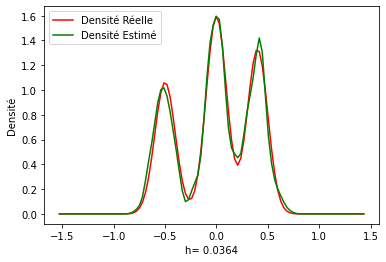
\includegraphics[width=13cm,height=8cm]{Figure 1.7.png}
  \caption{$h_N$  Optimal }
  \label{fig:$h_N$  Optimal}
\end{figure}
\newpage

L’estimation de la densité nécessite également le choix adéquat du paramètre de lissage $h_N$ , et pour cette valeur idéale, nous obtenons une allure qui suit parfaitement la vraie distribution. (Figure 1.7)
\section{Étude de la convergence}
L’étude théorique de la convergence de ${\hat f}_n$ (Densité estimée) vers $f$(Densité réelle) permet de formuler expression de $h_N$  optimal et de déterminer le noyau optimal censé à aboutir meilleure estimation.
Ainsi, évaluation de EQM mesure la différence entre densité estimée et densité réelle.
\begin{equation}
EQM=\text{var}({\hat f}_{n}) + \left(f - E[{\hat f}_n]\right)^2
\end{equation}
\myequations{Equation \ref{eq:Eq14}}
En minimisant EQM, nous obtiendrons l’expression analytique de la valeur optimale de $h_N$ notée $h^*_N$ comme suit : 
\begin{equation}
\fbox{\boldmath{$\displaystyle h^*_N = N^{-\frac{1}{5}} \cdot (J(f))^{-\frac{1}{5}} \cdot (M(K))^{\frac{1}{5}}
$}}
\end{equation}
\myequations{Equation \ref{eq:Eq14}}
Avec : 
\begin{align}
 J(f) &= \int_{-\infty}^{\infty} (f''(x))^2 \,dx \\ M(K) &= \int_{-\infty}^{\infty} K^2(u) \, du
\end{align}

$f''$  étant la dérivée seconde de $f$

L’expression théorique du paramètre de lissage optimal au sens de l'EQM dépend de la taille de l’échantillon $N$, de l’intégrale du noyau choisi élevé au carré $M(K)$ ainsi que de l’intégrale de la dérivée seconde élevée au carré de ${\hat f}_N$ notée $J(f)$. La valeur de $M(K)$, liée au noyau choisi, est facilement déduite analytiquement ou numériquement. Par contre, l’entité $J(f)$  ne peut être directement approchée puisqu’elle est liée à $f$, fonction inconnue à estimer.

\subsection{Optimisation de $J(f)$}
L'étude de la convergence de l'estimateur à noyau a permis de formuler l'expression théorique pour le pas optimal $h^*_N$. Cependant, il est difficile d'estimer l'intégrale de la dérivée seconde élevée au carré de la densité à estimer, appelée $J(f)$ . Pour résoudre ce problème, plusieurs méthodes ont été développées, telles que les méthodes ROT \shortcite{silverman1986, hardle1991smoothing,terrell1990variable} , cross-validation \shortcite{bowman1984,hall1987,Scott1987,Simon1991}, Plug-in \shortcite{hall1987,park1990} et la méthode des contrastes \shortcite{mugadi2004}. Ces méthodes cherchent à minimiser EQM en sélectionnant les paramètres de lissage optimaux. Nous allons voir par la suite les méthodes : LSCV, ROT et PLUG-IN et les comparer. 

\subsubsection{LSCV}
Simon Sheather a développé la méthode d'optimisation LSCV dans le contexte de l'estimation de densité au début des années 1991. L'idée de Sheather était d'utiliser la validation croisée\shortcite{bates2023crossvalidation} pour estimer le paramètre de largeur de bande optimal pour une estimation de densité de noyau. La méthode LSCV divise l'ensemble de données en deux parties, une partie pour l'estimation de densité et l'autre pour la validation. La partie de validation est utilisée pour calculer une fonction de perte, qui mesure l'erreur entre l'estimation de densité et les données observées. Le paramètre de largeur de bande qui minimise la fonction de perte est choisi comme le paramètre optimal pour l'estimation de densité.
\newline
\textbf{Sheather} a présenté la méthode LSCV et a montré qu'elle avait plusieurs avantages par rapport aux méthodes existantes de sélection de largeur de bande. En particulier, LSCV était plus robuste au choix de la fonction de noyau et pouvait être utilisé avec plusieurs fonctions de noyau, y compris celles qui n'étaient pas lisses ou symétriques.
Depuis la publication de l'article de Sheather, LSCV est devenu une méthode largement utilisée de sélection du paramètre de lissage dans le domaine de l'estimation de densité, et a été appliqué dans de nombreux contextes différents, notamment le traitement du signal, l'analyse d'image et la finance.
\begin{equation}
lscv(h)=\int \hat{f_{h^2}} - \frac{2}{n} {\sum_{i=1}^{n}{\hat f}_{-i}}(Xi)
\end{equation}
\myequations{Equation \ref{eq:Eq18}}
Voici une implémentation en Python 3 de la méthode LSCV : 
\begin{lstlisting}
import numpy as np
from sklearn.model_selection import GridSearchCV
#Mettre en place la grille des pas a explorer
param_grid = {'bandwidth': np.logspace(-1, 1, 20)}
#Utiliser GridSearchCV pour trouver le pas optimal
grid = GridSearchCV(KernelDensity(kernel='gaussian'), param_grid=param_grid, cv=10)
grid.fit(X[:, None])
hn_Optimal= grid.best_estimator_.bandwidth
\end{lstlisting}

\subsubsection{ROT}
La méthode de Silverman, nommée d'après le statisticien \textbf{David Silverman}, est une méthode non paramétrique utilisée pour estimer les fonctions de densité de probabilité. Elle a été introduite pour la première fois en 1986 dans un article intitulé \textbf{"Density Estimation for Statistics and Data Analysis"}. La méthode est largement utilisée dans l'analyse statistique et l'apprentissage automatique pour estimer les fonctions de densité de probabilité en raison de sa simplicité et de sa précision.

La méthode de Silverman repose sur l'hypothèse que la fonction de densité de probabilité sous-jacente est lisse et peut être approximée à l'aide d'une distribution gaussienne. La formule pour la méthode de Silverman consiste à sélectionner une largeur de bande optimale pour l'estimateur de densité de noyau gaussien en fonction des données disponibles. La largeur de bande optimale est choisie pour équilibrer le compromis entre la sur-lissage et le sous-lissage.

La méthode a été largement citée et appliquée dans divers domaines tels que l'économétrie, la finance et l'ingénierie. En fait, c'est la méthode implémentée par défaut dans la bibliothèque de KDE gaussien en Python. La méthode a également été étendue pour gérer les données multivariées et pour incorporer d'autres types de noyaux. Dans l'ensemble, la méthode ROT a été une contribution significative au domaine de l'estimation de densité non paramétrique et reste un outil important pour l'analyse des données.

Silverman a commencé par la formule de l'AMISE\footnote{L’AMISE fournit une mesure de l’efficacité d’un estimateur, et il est souvent utilisé pour comparer différents estimateurs en termes de performance à mesure que la taille de l’échantillon augmente.}  d'un estimateur $KDE$, qui implique la fonction de densité réelle $f(x)$  et la fonction noyau $K(x$) :
\begin{equation}
AMISE = \frac{1}{4} \int \frac{f''(x)^2}{[K(x)]^2} h^4 dx + \frac{1}{nh} \int [K(u)]^2 du
\end{equation}
\myequations{Equation \ref{eq:Eq19}}
Où $h$ est le paramètre de bande, n est la taille de l'échantillon et $f''(x)$ désigne la deuxième dérivée de $f(x)$ .

Silverman a ensuite fait deux hypothèses simplificatrices :
\begin{enumerate}
\item Il a supposé que la fonction noyau $K(x)$  est une distribution normale standard, ce qui signifie que l'intégrale de $K(u)^2$  sur son support est égale à $1$.
\item Il a supposé que la vraie fonction de densité $f(x)$  est lisse, ce qui signifie que sa deuxième dérivée est bornée.
\end{enumerate}

Sous ces hypothèses, le deuxième terme de la formule AMISE devient une constante, et Silverman s'est concentré sur la minimisation du premier terme par rapport à $h$ .En différenciant le premier terme par rapport à $h$ et en le fixant à zéro, il a obtenu la formule suivante pour le paramètre de bande optimal :
\begin{equation}
h_{Optimal} = 1.06 . \hat{\sigma} .  n^{\frac{-1}{5}}\end{equation}
\myequations{Equation \ref{eq:Eq20}}
Où  $\hat{\sigma}$ est l'écart-type de l'échantillon des données. Cette formule est connue sous le nom de règle de Silverman et elle fournit une méthode simple et pratique pour sélectionner le paramètre de bande dans KDE.

Voici une implémentation en Python 3 de la méthode ROT : 
\begin{lstlisting}
from scipy.stats import gaussian_kde
import numpy as np

kde = gaussian_kde(X)
evaluated = np.linspace(a, b, n)
density = kde(evaluated)

\end{lstlisting}
Comme nous l'avons précédemment dit ROT est la méthode implémentée par défaut dans la bibliothèque de KDE gaussien en Python.

\subsubsection{Plug-in}
Cette méthode fait appel à un algorithme itératif pour la recherche du pas optimal.

Le principe commence par un choix aléatoire de $J(f)$, ensuite les évaluations de $J(f)$  sont déduites à partir de la première valeur. Plusieurs itérations faites permettent de converger vers le paramètre de lissage optimal.

Étapes : 
\begin{enumerate}
    \item 	Détermination analytique de $M(K) $
	\item Choix arbitraire de $J_0(f)$, qui permet de la déduction de$h_N^0$
	\item Estimation de $f$ par la méthode de noyau en utilisant le paramètre de lissage $h_N^0$.\\Généralement cette première valeur, notée $f_0$, ne converge pas vers $f$.
	\item Ré-estimation de $J_k(f)$ en utilisant la dérivée seconde de ${\hat f}_{(k-1)}$ puis en l’intégrant. $h_N(k)$ est déduite à chaque itération.
	\item Arrêt de l’algorithme lorsque la différence entre $h_N^k$ et $h_N^{k-1}$ est relativement faible.

\end{enumerate}
Voici une implémentation en Python 3 de la méthode PLUG-IN à l’aide de l’estimateur de noyau : 
\begin{lstlisting}
def gitkernel(X,mini,maxi,r):
    P = 100
    P0 = 2000
    e = -100
    d = 100
    c = (2 * np.pi)**0.5
    I = 0
    for k in range(1, P0+1):
        zk = e + (d-e) * k/P0
        u = np.exp(-(zk**4)/4)
        I += u
    MK = I * (d-e) / (c*c*P0)
    Jf = 1
    n = len(X)


    for NBI in range(1,10):
        #Estimation de hN
        hn = (MK**0.2) * (Jf*n)**(-0.2)
        valeur=2*2.23*(hn)**(-6)/500;
        Y = []
        Yk = []
        for k in range(P):
            yk = mini + (maxi-mini)*k/P
            Y.append(0)
            Yk.append(yk)
            for i in range(1,n):
                z = (yk-X[i]) / hn
                z = z**2
                z = -0.5*z
                z = np.exp(z)
                Y[-1] += z
            Y[-1] = Y[-1] / (c*n*hn)
        e = -100
        d = 100
        I = 0
        Jf = 0
        z = 0
        for k in range(1, P-2):
            z = (Y[k+1]-2*Y[k]+Y[k-1])
            I += z**2
        I = I + ((Y[P-2])**2 + (Y[P-2]-2*Y[P-3])**2) / (r**4)
        #Estimation de Jf 
        Jf = I / (r**3)
        
    return Y


\end{lstlisting}

\section{Méthode de noyau difféomorphisme}
La méthode de noyau peut causer des problèmes (Effet de Gibbs) lorsque les observations sont rares aux bords de la plage, ce qui peut entraîner une sous-estimation de la densité de probabilité.
La solution consiste au changement de variable par un difféomorphisme $C^1$(Classe 1), qui nous aide à éliminer l’effet de Gibbs et bien estimer la densité.

Ensuite, nous introduisons un nouvel algorithme itératif pour l’ajustement de la valeur du paramètre de lissage. Le proposé algorithme, que nous appellerons Plug-in-difféomorphisme, s’inspire de l’algorithme Plug-in conventionnel lequel est adapté à cet estimateur.

Cette généralisation du Plug-in conventionnel nécessite une double initialisation ce qui rend sa convergence moins aisée.
L’expression de l’estimateur noyau difféomorphisme :
\begin{equation}
{\hat f}(x)= \frac{\left | \varphi '(x))  \right |}{Nh_N}\sum_{i=1}^{N}K(\frac{\varphi (x) - \varphi(X_i)}{h_N})
\end{equation}
\myequations{Equation \ref{eq:Eq21}}
Avec $\varphi$ est un $C^1$  difféomorphisme qui a pour limite l’infini lorsque $x$ tend vers $a$ ou $b$.

Exemple de $C^1$  difféomorphisme :
\newline
\begin{equation}
    \begin{cases}
\varphi _{a,b} : ]a,b[ \longrightarrow \mathbb{R} \\ x\longrightarrow log(\frac{x-a}{b-x})
\end{cases}
\end{equation}
\myequations{Equation \ref{eq:Eq22}}

Le choix du meilleur difféomorphisme a été effectué selon les valeurs de l’erreur quadratique moyenne qui doit être la plus faible possible.

\subsection{Optimisation du paramètre de lissage $(J_\phi (f)))$ : \\Plug-in Difféomorphisme }
La complexité de l'optimisation des paramètres de lissage pour la méthode de noyau \\difféomorphisme est accrue par l'utilisation de l'algorithme Plug-in, car$M_\phi(K)$ dépend de la densité de probabilité inconnue $f$, et $J_\phi(f)$ qui dépend de $f$,$f'$ et $f''$.\\En comparaison, l'algorithme Plug-in conventionnel utilise une constante $M(K)$ et $J(f)$ qui ne dépend que de $f''$.

En posant :		

$M_{\phi (K)} = M(K) \int _R \left|\varphi '(x) \right| f(x) \, dx$ 
\newline
et 
\newline
$J_{\phi}(f) = \int_{R} \frac{F^2 (x)}{[\varphi'(x)]^8} \, dx$
\newline
Il est possible de déduire la valeur de $h_N$ qui minimise l’EQM, que l’on notera $h^*_N$.

\begin{equation}
h^*_N = [M_\phi (K)]^\frac{1}{5} [J_\phi (f)]^\frac{-1}{5} N^\frac{-1}{5}
\end{equation}
\myequations{Equation \ref{eq:Eq23}}

Étapes:
\begin{enumerate}
    \item Initialisation arbitraire de $M_\phi^0 (K)$
    \item Initialisation arbitraire de $J_\phi^0 (K)$,  $h_N^0$ est déduite.
    \item Estimation de $f^0$ 
    \item A la $k^{eme}$ itération une approximation des différentes quantités :$ M_\phi (K)$ , ${f^{(k)}}' et {f^{(k)}}''$
    \item Estimation de $J_\phi$ $f^k$ ainsi de $h_N^k$
	\item Approximation de $f^{(k)}$  
	\item Arrêt de l’algorithme lorsque la différence entre $h_N^k$ et $h_N^{(k-1)}$ devient relativement faible.

\end{enumerate}
\newpage

\section{Conclusion}
	 Dans ce chapitre, nous avons commencé par expliquer la densité de probabilité et comment l’estimer, soit par des méthodes paramétriques ou non-paramétrique. Nous avons présenté les différentes méthodes non-paramétriques, mais nous nous sommes focalisés sur les estimateurs noyau, et par une étude de convergence nous avons bien minimisé le EQM et nous avons trouvé la fonction optimale du paramètre de lissage, en utilisant l’algorithme plug-in qui permet de converger la densité estimée vers la densité réelle. 

Après, nous avons introduit la méthode noyau difféomorphisme et l’algorithme plug-in difféomorphisme pour une meilleure estimation des distributions à supports bornés ou semi-bornés. Cette méthode présente l’avantage de minimiser de manière remarquable le phénomène de Gibbs. Mais nous avons constaté une augmentation de complexité de l’algorithme qui sert à l’optimisation de paramètre de lissage, algorithme Plug-in.
